\section{User Interfaces}
\label{sec:interface}

For the semi-autonomous vehicles defined above to be able to interact
with the IM, we need to define interfaces for passing control from the
human to the driver agent and back.  Safety is a common (and quite
reasonable) concern when involving human drivers in the control loop
of autonomous vehicles.  In the semi-autonomous vehicles we introduced
in the previous section, a human driver can always intervene and
simply follow the traffic signal. In this section, we describe how our
proposed protocol can be realized safely, as long as no driver runs a
red light (without a reservation granted).

For drivers of vehicle types SA-ACC, SA-CC, and SA-Com, we assume
inclusion in the vehicle of a single button that signals the driver
agent to ask for a reservation.  We define such an active ``opt-in''
interface so as to allow drivers to drive as they do today if they do
not signal their intention for a semi-autonomous reservation.  It is
also important that there is a clear indicator (such as a green light)
installed in the car which indicates when the request has been
confirmed.  The driver must then actively pass control to the
computer, again by pressing the single button.  In this way, the
driver will not be surprised by any sudden autonomous actions of the
vehicle.  Figure~\ref{fig:interaction} shows the interactions between
human drivers, driver agents, and the Intersection Manager.
Since vehicles are semi-autonomous, only some control will be passed
to the driver agent when the vehicle is passing the intersection.

\begin{figure}[t]
\centering
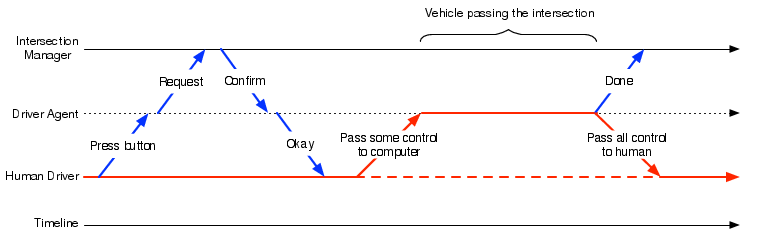
\includegraphics[width=\columnwidth]{figures/interaction}
\caption{The interactions between human drivers, driver agents, and
the Intersection Manager.}
\label{fig:interaction}
\end{figure}

In Type SA-Com vehicles, the driver can safely enter the intersection
when the request is confirmed. If the request is confirmed and the
driver decides not to enter, it still does no harm (even though the
tiles it requested are wasted).  When the reservation is granted to
Types SA-ACC and SA-CC vehicles, the vehicle starts controlling the
speed.  If the person touches the brakes or accelerator, the person
regains control, and the reservation is cancelled.

There is a point near the entry of the intersection where it is no
longer possible to brake before entering the intersection. Beyond this
point, the person must lose the ability to take back control of the
speed until leaving the intersection (presumably with an emergency
override option for extreme situations).  This constraint is based on
the fact that if the driver were to change its velocity, its
reservation would need to be modified.  The IM cannot guarantee that
the modified reservation will be confirmed.

Drivers can must always steer in type SA-CC vehicles. For type SA-ACC,
the vehicle might follow a vehicle in front of it to make a turn. The
driver would cede control over the steering wheel in this case.

Two points are important to keep in mind about all the cases above:
\begin{itemize}

\item The only actions a human driver needs to take is to press a
single button to request a reservation, and press a single button to
accept it (possibly the same button).  All of the negotiation
involving arrival times and trajectories is completed automatically by
the driver agent and IM in a manner similar to how it is done in AIM.

\item No equipment is \emph{required} on any car.  Like FCFS-Signal in
AIM, Semi-AIM is fully compatible with ``classic'' human-driven cars
that have no communications equipment.

\end{itemize}

% \commentp{It would be useful in this section to add a flowchart or
% some other representation of how and when control passes between the
% car and the person.}

% \section{Definitions}

% A road $r$ consists a finite number of lanes $l_1$, $l_2$, \ldots,
% $l_n$.  We write $r = (1_1, l_2, \ldots l_n)$.
% All lanes in a road are in the same direction.
% An \emph{entry} road of an intersection is a road
% from which traffic flows into the intersection.
% An \emph{exit} road is a road from which traffic flows out of
% an intersection.


% \section{A General AIM architecture}

% We generalize the AIM architecture as follows.

% \commentc{Maybe draw a diagram to show to how AIM works}

% This framework can be considered as an extension to AIM.
% In AIM, each request is a $4$-tuple $\langle t, v, l_1, l_2 \rangle$.
% \commentc{Fit AIM requests into the next framework.}

% In AIM, these values are *exact*. However, in SemiAIM,
% these values can be constrained.

% No need to think about the acceleration schedule yet.

% In essence, no human intervention is involved in the control loop.


%%% Local Variables: 
%%% mode: latex
%%% TeX-master: "main"
%%% End:
